\subsection{Heuristic vs. the Exact Solver}\label{sec:heuristic-vs-optimal}

We implemented the ILP of Section~\ref{sec:formulation} in IBM CPLEX and use it
both as the optimal baseline and to expose why a heuristic is needed. Two
properties matter: the exact solver does not scale, and MASMAN stays close to its
optimum where it does.

\textbf{Scalability.} Table~\ref{tbl:exact-runtime-topology} reports the optimal
solve time as the fat-tree degree grows, for a fixed load of 8 chains: it rises
from 4~s at \(k = 6\) to 5~min~20~s at \(k = 12\). Fixing the topology at a
12-ary fat tree and increasing the load instead
(Table~\ref{tbl:exact-runtime-chains}), the solve time grows from 5~min~20~s at 8
chains to 16~min~33~s at 11 chains, and exhausts the 12~GB heap (out-of-memory) at
12 chains. The exact solver is therefore confined to small instances, whereas the
heuristic places hundreds of chains (Section~\ref{sec:joint-vs-disjoint}). These
runtimes were measured on 4~vCPUs with 16~GB of RAM and a 12~GB heap, with no
constraint on the VNFM license fee.

\begin{table}[H]
\caption{Optimal solve time vs. fat-tree degree \(k\) (8 chains).}
\label{tbl:exact-runtime-topology}
\begin{tabularx}{0.6\textwidth}{Xr}
\toprule
\textbf{\(k\)-ary fat tree} & \textbf{Time} \\
\midrule
6 & 4 s \\
8 & 7 s \\
10 & 1 min \\
12 & 5 min 20 s \\
\bottomrule
\end{tabularx}
\end{table}

\begin{table}[H]
\caption{Optimal solve time vs. number of chains (12-ary fat tree, 4~vCPU /
16~GB).}
\label{tbl:exact-runtime-chains}
\begin{tabularx}{0.6\textwidth}{Xr}
\toprule
\textbf{Chains} & \textbf{Time} \\
\midrule
8 & 5 min 20 s \\
10 & 7 min 6 s \\
11 & 16 min 33 s \\
12 & out of memory \\
\bottomrule
\end{tabularx}
\end{table}

\textbf{Near-optimality.} On instances the exact solver can handle, we report the
heuristic revenue as a proportion of the optimal revenue
(Table~\ref{tbl:near-optimal}), for 100 chains of length 5--7 at two per-instance
revenue ranges. The management-aware VNF placement reaches 81\% of optimal and the
full method (with Tabu VNFM consolidation) reaches 82\%, against 61\% for the
unmodified Bari~\cite{Bari2015} baseline. The advantage widens as the per-instance
revenue grows, i.e. as accepting each chain becomes more valuable relative to the
VNFM license cost.

\begin{table}[H]
\caption{Heuristic revenue as a percentage of the optimal revenue (100 chains,
length 5--7).}
\label{tbl:near-optimal}
\begin{tabularx}{\textwidth}{Xrrr}
\toprule
\textbf{Revenue per instance} & \textbf{Bari~\cite{Bari2015}} & \textbf{MASMAN (VNF phase)} & \textbf{MASMAN (full)} \\
\midrule
10--20 & 60\% & 65\% & 68\% \\
15--25 & 61\% & 81\% & 82\% \\
\bottomrule
\end{tabularx}
\end{table}

\subsection{Joint vs. Disjoint}\label{sec:joint-vs-disjoint}

We compare the \emph{joint} solution (placing VNFs and their VNFM together)
against the \emph{disjoint} baseline (placing VNFs first and the VNFM afterward),
both solved to optimality with CPLEX. The key effect is one of \emph{feasibility}:
a management-blind disjoint placement can strand whole chains because no
admissible VNFM exists for the chosen VNF layout, so the joint solution accepts
more chains. Crucially, this benefit is \emph{conditional}---it appears only when
the management constraints actually bind, as the two topologies below make clear.
We therefore report chain \emph{acceptance rate} as the primary metric; the
corresponding mean revenue, which only smooths over the mechanism, is tabulated
for reference in Appendix~\ref{sec:revenue-appendix}. We vary the number of
chains; chains are generated randomly with the configuration in
Table~\ref{tbl:chain-config}.

\begin{table}[H]
\caption{Chain configuration.}
\label{tbl:chain-config}
\begin{tabularx}{0.6\textwidth}{lX}
\toprule
\textbf{Property} & \textbf{Value} \\
\midrule
Length & \([4, 7)\) \\
Per-instance cost & \$100 \\
Bandwidth & 250 bps \\
\bottomrule
\end{tabularx}
\end{table}

We evaluate two topologies: a FatTree with \(k = 6\), and a USNet topology with
3--4 nodes attached to each of its points. Each point is the average of 15 CPLEX
runs under a time limit and a 5\% optimality-gap limit.

\subsection{Acceptance Rate: the Feasibility Effect}\label{sec:acceptance}

We report chain \emph{acceptance rate}---the fraction of requested chains that
are admitted---and test each point with a paired Wilcoxon signed-rank test (joint
vs. disjoint on the \emph{same} chain set, 10--15 runs per point).

Two facts stand out. First, the joint solution accepts \(\approx 100\%\) of
chains in \emph{every} regime---it is essentially feasibility-immune, because it
placed the VNFs with management in mind. Second, the disjoint baseline is
\emph{bimodal}: a run either nearly succeeds or collapses, because the post-hoc
manager step is infeasible for the layout the VNF stage happened to choose. The
per-point coefficient of variation (Disjoint CV, up to \(\sim\)80\%) and the
worst single run (Disjoint min, as low as 0\%) expose a spread that the revenue
averages hide. All revenue differences below are significant at \(p < 0.05\)
(paired Wilcoxon).

\begin{table}[H]
\caption{Chain acceptance rate on FatTree (\(k = 6\), default VNFM)---management
binds.}
\label{tbl:acceptance-fattree}
\begin{tabularx}{\textwidth}{Xrrrr}
\toprule
\textbf{Chains} & \textbf{Joint (\%)} & \textbf{Disjoint (\%)} & \textbf{Disjoint min (\%)} & \textbf{Disjoint CV (\%)} \\
\midrule
10 & 100.0 & 46.0 & 0.0 & 69.6 \\
15 & 100.0 & 18.7 & 0.0 & 62.8 \\
20 & 100.0 & 20.3 & 5.0 & 41.6 \\
25 & 100.0 & 31.2 & 8.0 & 78.9 \\
30 & 100.0 & 60.2 & 6.7 & 55.3 \\
35 & 100.0 & 85.7 & 77.1 & 7.0 \\
40 & 100.0 & 83.2 & 62.5 & 15.4 \\
45 & 100.0 & 87.7 & 44.4 & 19.8 \\
50 & 99.9 & 70.5 & 36.0 & 39.3 \\
55 & 100.0 & 61.5 & 23.6 & 47.6 \\
60 & 99.9 & 56.4 & 28.3 & 46.8 \\
65 & 99.9 & 65.6 & 29.2 & 47.6 \\
70 & 100.0 & 53.2 & 25.7 & 53.9 \\
75 & 99.8 & 53.6 & 32.0 & 51.7 \\
80 & 100.0 & 56.0 & 33.8 & 46.2 \\
85 & 100.0 & 50.6 & 31.8 & 48.5 \\
90 & 100.0 & 59.6 & 27.8 & 46.6 \\
\bottomrule
\end{tabularx}
\end{table}

\begin{table}[H]
\caption{Chain acceptance rate on USNet (4-hop manager radius)---management
binds.}
\label{tbl:acceptance-usnet-radius}
\begin{tabularx}{\textwidth}{Xrrrr}
\toprule
\textbf{Chains} & \textbf{Joint (\%)} & \textbf{Disjoint (\%)} & \textbf{Disjoint min (\%)} & \textbf{Disjoint CV (\%)} \\
\midrule
10 & 100.0 & 34.7 & 0.0 & 80.8 \\
15 & 100.0 & 41.8 & 26.7 & 24.4 \\
20 & 100.0 & 42.3 & 25.0 & 22.8 \\
25 & 100.0 & 45.1 & 24.0 & 45.4 \\
30 & 99.8 & 68.7 & 40.0 & 33.0 \\
35 & 100.0 & 94.1 & 85.7 & 4.5 \\
40 & 99.8 & 85.3 & 72.5 & 9.8 \\
45 & 99.9 & 87.1 & 57.8 & 12.6 \\
50 & 99.9 & 93.6 & 88.0 & 2.7 \\
55 & 99.6 & 89.8 & 58.2 & 10.2 \\
60 & 99.6 & 90.3 & 81.7 & 4.3 \\
65 & 99.3 & 88.2 & 47.7 & 12.7 \\
70 & 99.8 & 92.1 & 87.1 & 3.6 \\
75 & 99.4 & 87.7 & 46.7 & 12.8 \\
80 & 99.4 & 91.4 & 86.2 & 3.1 \\
85 & 99.2 & 90.6 & 60.0 & 9.3 \\
90 & 99.3 & 91.7 & 88.9 & 2.1 \\
\bottomrule
\end{tabularx}
\end{table}

\begin{table}[H]
\caption{Chain acceptance rate on USNet (default VNFM)---management slack.}
\label{tbl:acceptance-usnet-slack}
\begin{tabularx}{\textwidth}{Xrrrr}
\toprule
\textbf{Chains} & \textbf{Joint (\%)} & \textbf{Disjoint (\%)} & \textbf{Disjoint min (\%)} & \textbf{Disjoint CV (\%)} \\
\midrule
50 & 100.0 & 100.0 & 100.0 & 0.0 \\
75 & 100.0 & 100.0 & 100.0 & 0.0 \\
100 & 100.0 & 100.0 & 100.0 & 0.0 \\
125 & 100.0 & 100.0 & 100.0 & 0.0 \\
150 & 99.9 & 100.0 & 100.0 & 0.0 \\
\bottomrule
\end{tabularx}
\end{table}

\begin{figure}[H]
\centering
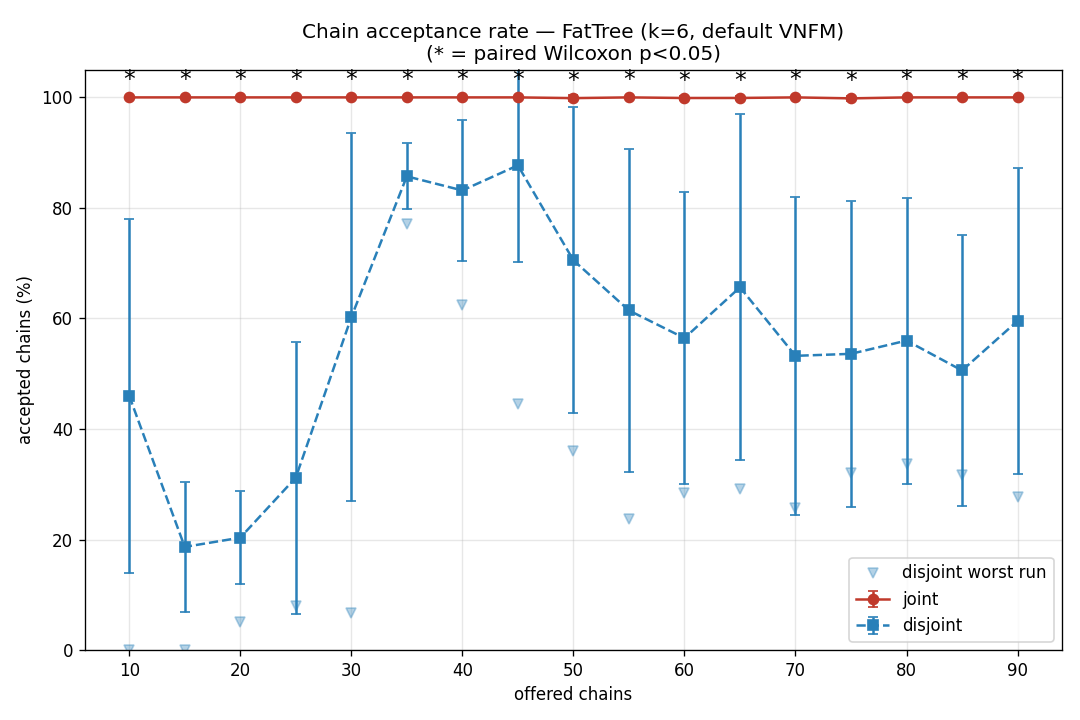
\includegraphics[width=0.32\textwidth]{plots/acceptance-fattree.png}
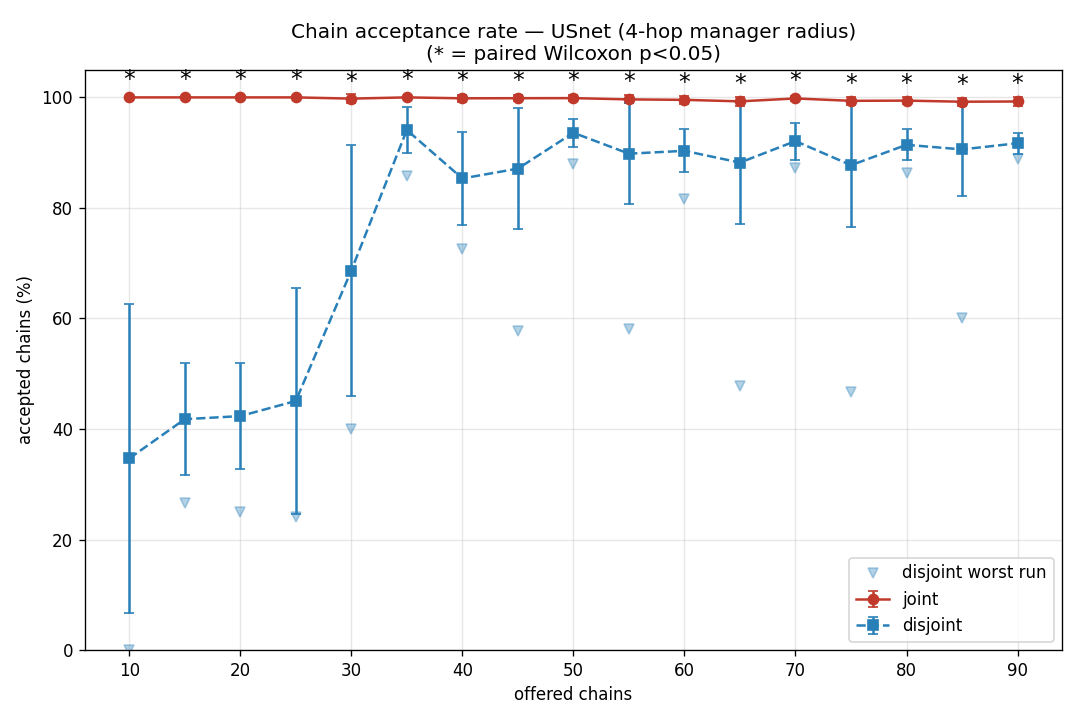
\includegraphics[width=0.32\textwidth]{plots/acceptance-usnet-radius.png}
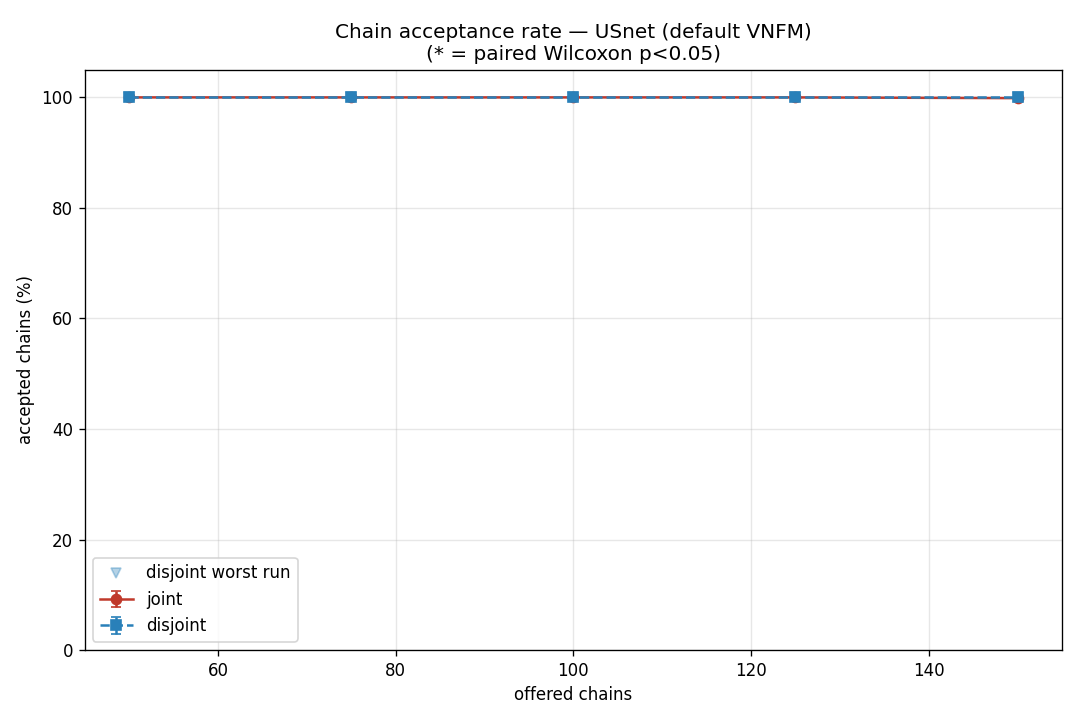
\includegraphics[width=0.32\textwidth]{plots/acceptance-usnet-slack.png}
\caption{Acceptance rate vs. number of chains. Left: FatTree (default VNFM).
Middle: USNet (4-hop radius). Right: USNet (slack management). Joint stays at
\(\approx 100\%\); disjoint collapses precisely where management binds and matches
joint where it does not.}
\label{fig:acceptance}
\end{figure}

On FatTree with the default VNFM, and on USNet once a 4-hop manager radius is
imposed, the management constraint binds and joint placement dominates. In the
slack regime (USNet, default VNFM) disjoint reaches 100\% acceptance with zero
variance, so the joint formulation adds nothing---and, accounting for management
that never binds, it diverts VNF placement enough to be \emph{marginally worse}
on revenue (\(-0.2\%\) to \(-0.9\%\), paired Wilcoxon \(p < 0.01\); see
Appendix~\ref{sec:revenue-appendix}). We keep this null result in deliberately:
it delimits the regime in which joint placement is worth the extra coupling. Note
that the same USNet topology moves from ``no difference'' to a clear joint
advantage by tightening a single management parameter---the manager radius---which
is the central message of this comparison.

\subsection{When Joint Placement Matters: a Controlled Sweep}\label{sec:sweep}

The comparisons above show \emph{that} the advantage is conditional; a controlled
sweep on the 15-node example topology isolates \emph{why}. Here the joint method
is the management-aware heuristic (Bari) and the disjoint method is the same
pipeline with management-blind VNF placement, with 8 paired runs per point.

\textbf{The management constraint is the cause.} Holding the network and chains
fixed, we toggle the per-node co-location (notManagerNodes) management constraint
on and off (Table~\ref{tbl:sweep-constraint}, Figure~\ref{fig:sweep-constraint}).
With it \emph{on}, the joint method leads disjoint by 12--19 percentage points of
acceptance at low load; with it \emph{off}, disjoint matches joint exactly (gap 0)
at every load. Joint acceptance is identical in both columns---it is immune by
construction. The gap also decays to 0 as load rises and raw VNF resources, not
management, become the bottleneck.

\begin{table}[H]
\caption{Toggling the management constraint (controlled A/B). The joint advantage
exists if and only if the constraint binds, and decays under load.}
\label{tbl:sweep-constraint}
\begin{tabularx}{\textwidth}{Xrrrrr}
\toprule
\textbf{Load} & \textbf{Joint (\%)} & \textbf{Disjoint on (\%)} & \textbf{Gap on} & \textbf{Disjoint off (\%)} & \textbf{Gap off} \\
\midrule
2 & 100.0 & 87.5 & 12.5 & 100.0 & 0.0 \\
3 & 100.0 & 83.3 & 16.7 & 100.0 & 0.0 \\
4 & 100.0 & 81.2 & 18.8 & 100.0 & 0.0 \\
5 & 100.0 & 82.5 & 17.5 & 100.0 & 0.0 \\
6 & 93.8 & 77.1 & 16.7 & 93.8 & 0.0 \\
7 & 87.5 & 75.0 & 12.5 & 87.5 & 0.0 \\
8 & 78.1 & 73.4 & 4.7 & 78.1 & 0.0 \\
9 & 70.8 & 69.4 & 1.4 & 70.8 & 0.0 \\
10 & 63.8 & 62.5 & 1.2 & 63.8 & 0.0 \\
12 & 54.2 & 54.2 & 0.0 & 54.2 & 0.0 \\
\bottomrule
\end{tabularx}
\end{table}

\begin{figure}[H]
\centering
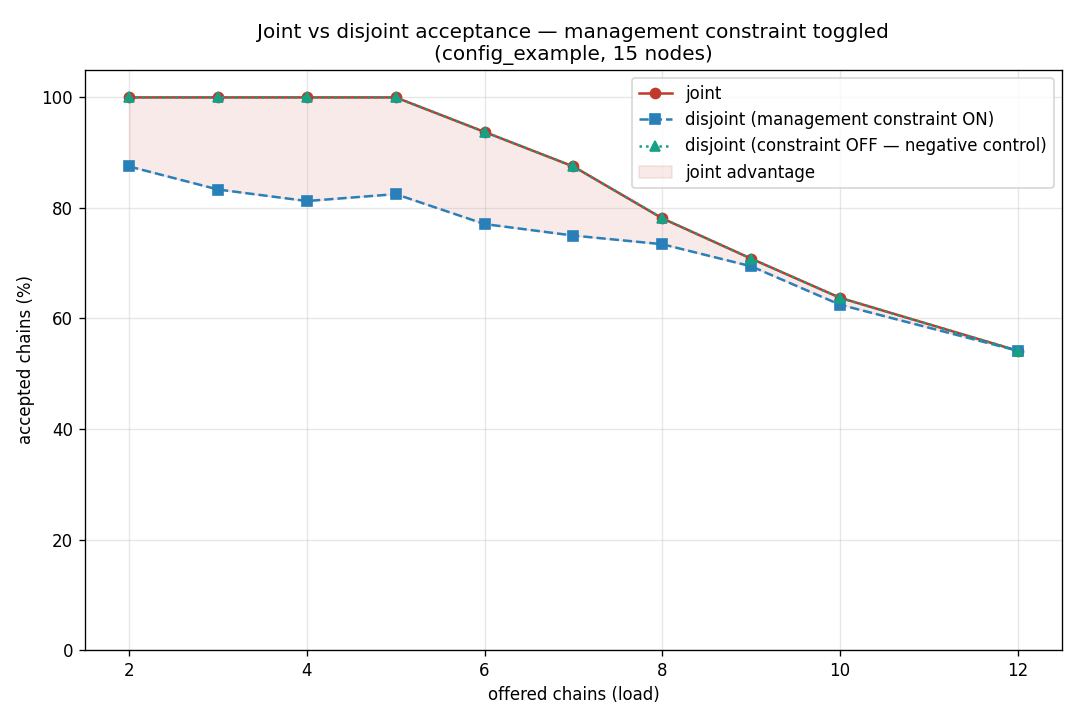
\includegraphics[width=0.7\textwidth]{plots/sweep-constraint.png}
\caption{Acceptance vs. load with the management constraint on vs. off. The
joint--disjoint gap appears only when the constraint is present.}
\label{fig:sweep-constraint}
\end{figure}

\textbf{Manager capacity is not the lever (negative control).} Sweeping manager
capacity over two orders of magnitude barely moves the gap
(Table~\ref{tbl:sweep-capacity}): on this topology capacity does not bind, so it
is not what drives the joint advantage. The binding lever here is the co-location
constraint; on the full topologies it is the manager radius
(Section~\ref{sec:acceptance}).

\begin{table}[H]
\caption{Manager capacity as a non-binding lever (negative control). The gap is
essentially constant from capacity 1 to 100.}
\label{tbl:sweep-capacity}
\begin{tabularx}{0.7\textwidth}{Xrrr}
\toprule
\textbf{Capacity} & \textbf{Joint (\%)} & \textbf{Disjoint (\%)} & \textbf{Gap (pp)} \\
\midrule
1 & 93.8 & 77.1 & 16.7 \\
2 & 93.8 & 81.2 & 12.5 \\
3 & 93.8 & 77.1 & 16.7 \\
5 & 93.8 & 81.2 & 12.5 \\
10 & 93.8 & 77.1 & 16.7 \\
20 & 93.8 & 77.1 & 16.7 \\
100 & 93.8 & 79.2 & 14.6 \\
\bottomrule
\end{tabularx}
\end{table}

Together these results turn a soft comparison into a characterization: joint
placement does not make good layouts better; it makes infeasible layouts
feasible---exactly when a management constraint binds, and not otherwise.
